\documentclass[11pt,a4paper]{article}

% --- Core Geometry and Encoding (pdfLaTeX & Vietnamese Support) ---
\usepackage[utf8]{inputenc}
\usepackage[vietnamese,english]{babel}
\usepackage[T5,T1]{fontenc}
\usepackage{lmodern}
\usepackage[top=2cm, bottom=2.5cm, left=2cm, right=2cm]{geometry}

% --- Math, Graphics and Technical Packages ---
\usepackage{amsmath, amssymb, amsfonts}
\usepackage{booktabs}
\usepackage{tabularx}
\usepackage{enumitem}
\usepackage{graphicx}
\usepackage{subcaption}
\usepackage{float}
\usepackage{hyperref}
\usepackage{xcolor}

\hypersetup{
	colorlinks=true,
	linkcolor=blue!80!black,
	citecolor=blue!80!black,
	urlcolor=blue!70!black
}

\setlist[itemize]{leftmargin=1.5em, itemsep=2pt, topsep=3pt}
\setlist[enumerate]{leftmargin=1.5em, itemsep=2pt, topsep=3pt}

\begin{document}
	
	% ==================== HEADER ====================
	\begin{center}
		{\fontsize{10}{12}\selectfont \textbf{VIETNAM NATIONAL UNIVERSITY HO CHI MINH CITY (VNU-HCM)}} \\
		{\fontsize{10}{12}\selectfont \textbf{UNIVERSITY OF SCIENCE (HCMUS)}} \\
		{\fontsize{9.5}{11.5}\selectfont FACULTY OF INFORMATION TECHNOLOGY} \\
		{\fontsize{9.5}{11.5}\selectfont ADVANCED PROGRAM IN COMPUTER SCIENCE (APCS)} \\[0.4em]
		{\fontsize{11}{13}\selectfont \textbf{COURSE: SC203 -- SCIENTIFIC METHOD}} \\[0.2em]
		\rule{\textwidth}{0.8pt}
	\end{center}
	
	\vspace{0.3em}
	
	% ==================== TITLE ====================
	\begin{center}
		{\Large \textbf{Mathematical Information Retrieval (MathIR)}} \\[0.4em]
		{\normalsize \textit{Topic: Identifying Critical Bottlenecks and Failure Modes in Prior Literature}}
	\end{center}
	
	\vspace{0.4em}
	
	% ==================== STUDENT RESEARCH TEAM ====================
	\begin{center}
		\textbf{\large Research Team (Group 2)} \\[0.4em]
		\begin{tabular}{ll}
			\toprule
			\textbf{Student ID} & \textbf{Full Name} \\
			\midrule
			25125024 & \foreignlanguage{vietnamese}{Đỗ Viết Hoàng Long} \\
			25125091 & \foreignlanguage{vietnamese}{Trần Đức Toàn}    \\
			25125010 & \foreignlanguage{vietnamese}{Phạm Trung Duy}   \\
			25125006 & \foreignlanguage{vietnamese}{Nguyễn Nguyễn Gia Bảo} \\
			\bottomrule
		\end{tabular}
		\\[0.5em]
		\textbf{Instructor:} Assoc. Prof. Dr. \foreignlanguage{vietnamese}{Trần Minh Triết} \quad | \quad 
		\textbf{Supervisor:} \foreignlanguage{vietnamese}{Thầy Huỳnh Viết Thám} \\[0.2em]
		\textbf{Project Repository:} \url{https://github.com/Dvhlong55/MathIR}
	\end{center}
	
	\vspace{0.4em}
	\hrule
	\vspace{0.8em}
	
	% ==================== ABSTRACT / EXECUTIVE SUMMARY ====================
	\begin{abstract}
		In this empirical progress report, Group 2 investigates the practical retrieval boundaries of three established paradigms in Mathematical Information Retrieval (MathIR): pre-trained neural language models (MathBERT), tree-based structural embeddings (Tangent-CFT), and symbolic computer algebra systems (SymPy CAS). Through an interactive adversarial test suite running on live weights, we primarily dissect the critical failure modes of deep neural transformers. Our findings demonstrate that MathBERT exhibits severe semantic blindness to polarity reversals ($x > 0$ vs. $x < 0$ at 93.0\% similarity), fraction inversions ($\frac{x}{y}$ vs. $\frac{y}{x}$ at 99.0\%), algebraic misconceptions ($(a+b)^2$ vs. $a^2+b^2$ at 93.4\%), and orthogonal trigonometric functions ($\sin(x)$ vs. $\cos(x)$ at 93.6\%), while experiencing a sharp degradation when processing Vietnamese mathematical statements (dropping to 57.6\%). Furthermore, when handling informal sequence statements ($1+2+..+n$), CAS suffers catastrophic syntax crashes. Consequently, we formulate a multi-stage Neuro-Symbolic Hybrid architecture that cascades neural semantic recall with structural verification filters.
	\end{abstract}

	% ==================== SECTION 1: INTRODUCTION & SETUP ====================
	\section{Introduction and Experimental Setup}
	Mathematical Information Retrieval (MathIR) requires capturing both semantic domain context and exact algebraic structure. Existing research predominantly isolates methods into either pure deep representation learning or rigid structural matching. To establish rigorous empirical grounding for our research project, we deployed an interactive local benchmark workbench integrating three official baseline engines:
	
	\begin{enumerate}
		\item \textbf{Neural Baseline (MathBERT):} Official 110M parameter pre-trained Transformer checkpoint (12 layers, 768 hidden dimensions) pre-trained on arXiv mathematical corpora by Peng et al. (2021). Cosine similarity of dense embeddings serves as the continuous semantic distance metric.
		\item \textbf{Structural Baseline (Tangent-CFT AST):} Operator Tree (OPT) parser extracting spatial triplet tuples $(Operator, Operand, Position)$ evaluated via Jaccard/Dice structural overlap coefficients (Mansouri et al., SIGIR 2019).
		\item \textbf{Symbolic Baseline (SymPy CAS):} Deterministic Computer Algebra System evaluating algebraic zero-difference reductions ($\Delta = f_A - f_B = 0$).
	\end{enumerate}

	% ==================== SECTION 2: NEURAL BASELINE FAILURE MODES ====================
	\section{Empirical Evaluation of Neural Architecture (MathBERT)}
	While MathBERT achieves competitive benchmark numbers on generic text retrieval, adversarial mathematical stress testing reveals fundamental structural blind spots stemming from 1D subword serialization.

	\subsection{Polarity and Ratio Inversion Blindness}
	In mathematical problem solving, bounding domains define completely incompatible solution spaces. When querying opposite inequalities ($x > 0$ vs. $x < 0$), MathBERT assigns a deceptive \textbf{93.0\%} similarity score (Figure~\ref{subfig:inequality}). Similarly, reversing numerator and denominator in a ratio represents a reciprocal transformation ($f_A = 1/f_B$), yet MathBERT reports \textbf{99.0\%} equivalence (Figure~\ref{subfig:fraction}).

	\begin{figure}[!htbp]
		\centering
		\begin{subfigure}[b]{0.485\textwidth}
			\centering
			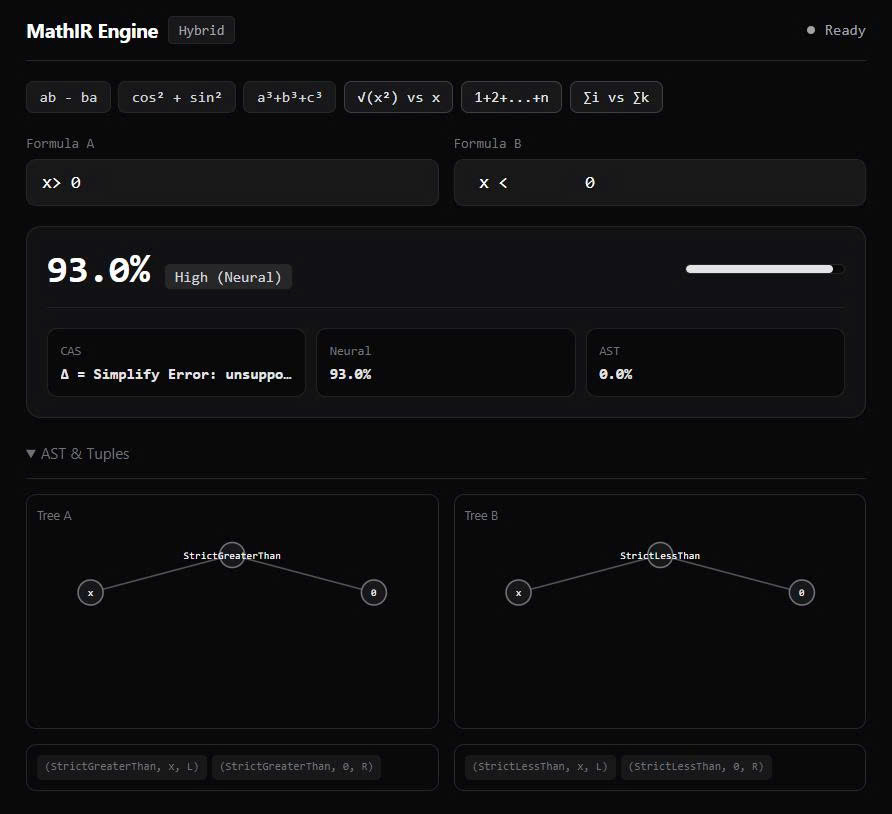
\includegraphics[width=\textwidth]{figures/fig_inequality.jpg}
			\caption{Inequality direction ($x > 0$ vs. $x < 0$, 93.0\%).}
			\label{subfig:inequality}
		\end{subfigure}
		\hfill
		\begin{subfigure}[b]{0.485\textwidth}
			\centering
			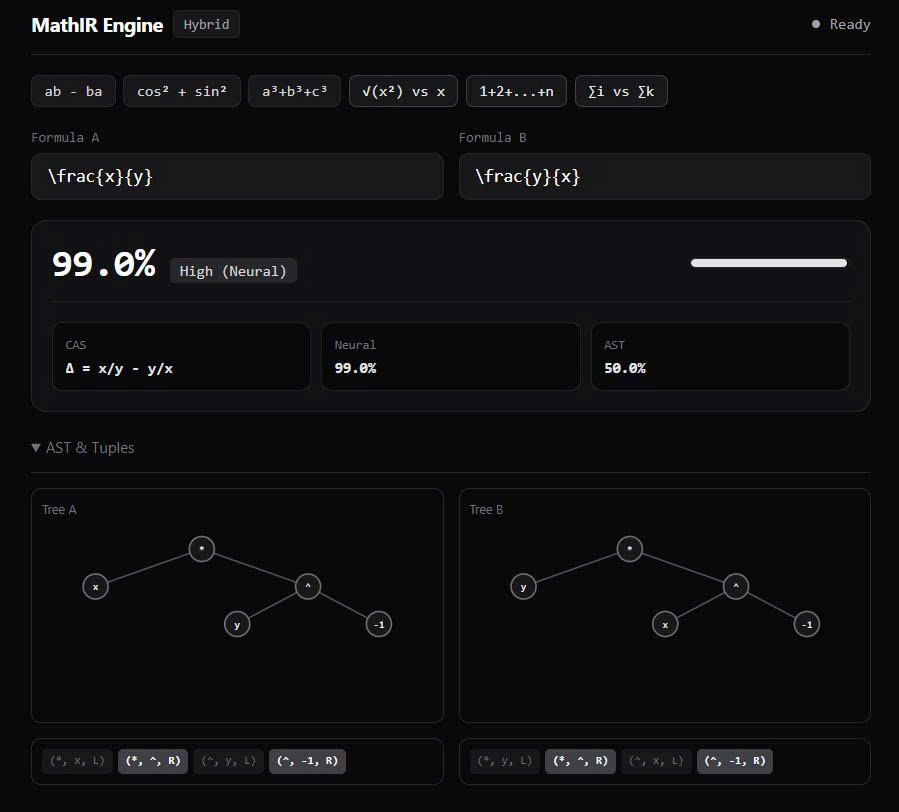
\includegraphics[width=\textwidth]{figures/fig_fraction.jpg}
			\caption{Fraction inversion ($\frac{x}{y}$ vs. $\frac{y}{x}$, 99.0\%).}
			\label{subfig:fraction}
		\end{subfigure}
		\caption{Adversarial testing on polarity and ratio inversions: MathBERT exhibits critical semantic blindness due to identical subword attention patterns.}
		\label{fig:polarity_fraction}
	\end{figure}

	\noindent \textbf{Theoretical Cause:} Self-attention layers treat tokens `$x$', `$y$', and relational operators symmetrically, while 1D positional encodings fail to resolve the 2D hierarchical numerator-denominator distinction.

	\subsection{Algebraic Fallacies and Orthogonal Trigonometric Confusion}
	A notorious high-school algebra fallacy equates $(a+b)^2$ with $a^2 + b^2$, disregarding the cross term $2ab$. MathBERT scores this pair at \textbf{93.4\%} (Figure~\ref{subfig:algebra}), whereas CAS correctly identifies the non-zero discrepancy $\Delta = 2ab$. Furthermore, when evaluating orthogonal trigonometric basis functions with a $\pi/2$ phase shift ($\sin(x)$ vs. $\cos(x)$), MathBERT erroneously scores \textbf{93.6\%} similarity (Figure~\ref{subfig:trig}), despite their functional orthogonality ($\int_0^{2\pi} \sin(x)\cos(x) dx = 0$) and zero AST overlap (0.0\%).

	\begin{figure}[!htbp]
		\centering
		\begin{subfigure}[b]{0.485\textwidth}
			\centering
			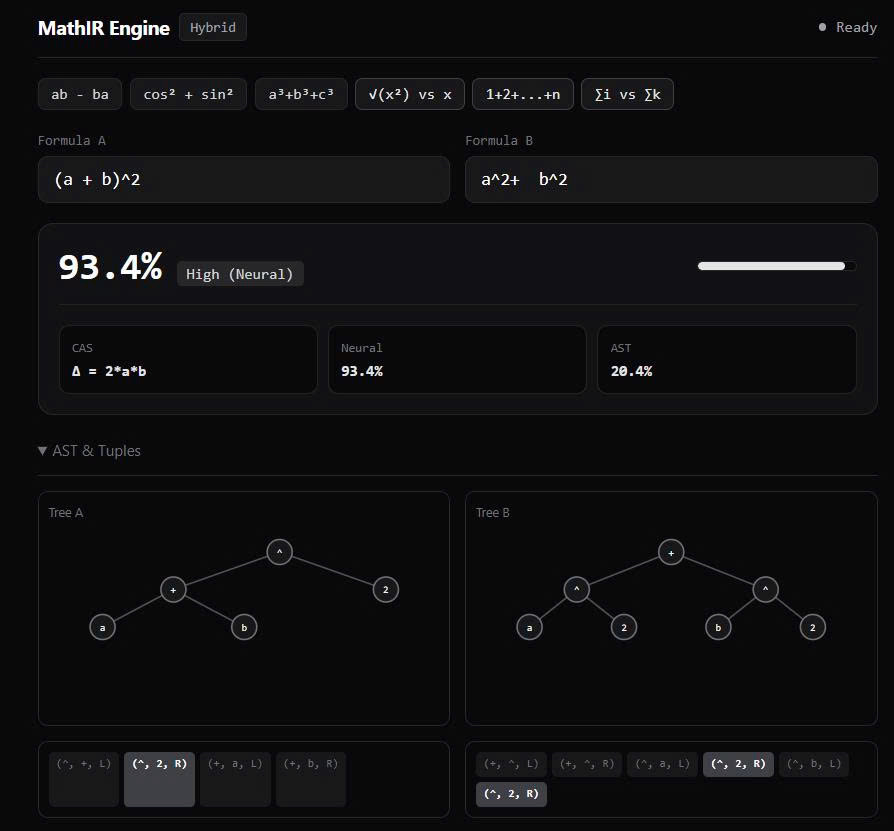
\includegraphics[width=\textwidth]{figures/fig_algebra.jpg}
			\caption{Algebraic fallacy ($(a+b)^2$ vs. $a^2 + b^2$, 93.4\%).}
			\label{subfig:algebra}
		\end{subfigure}
		\hfill
		\begin{subfigure}[b]{0.485\textwidth}
			\centering
			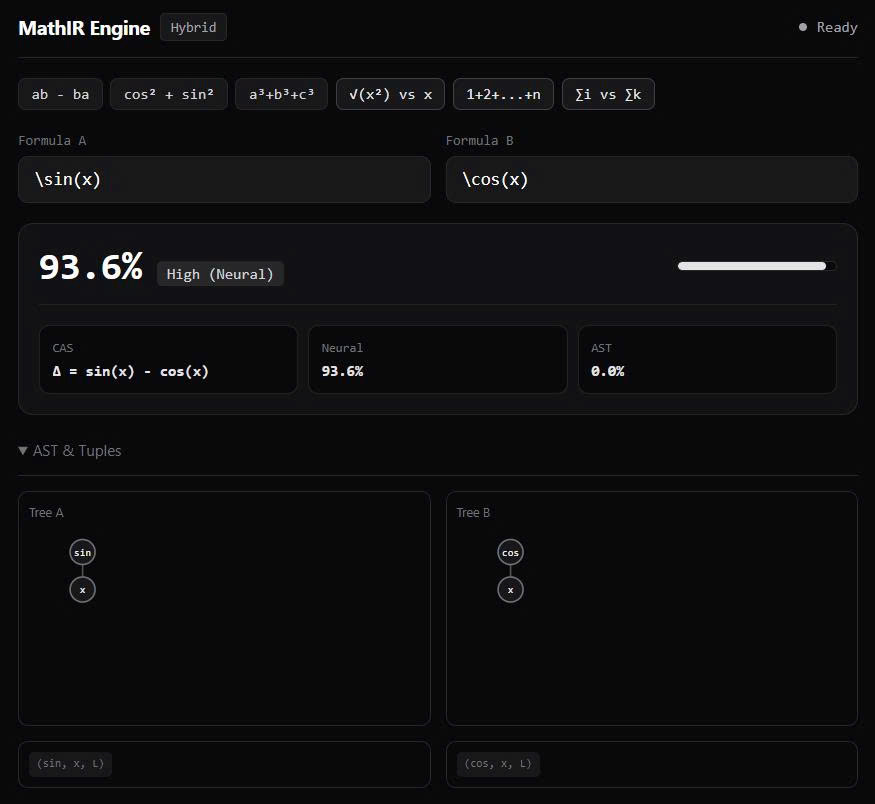
\includegraphics[width=\textwidth]{figures/fig_trig.jpg}
			\caption{Trigonometric confusion ($\sin(x)$ vs. $\cos(x)$, 93.6\%).}
			\label{subfig:trig}
		\end{subfigure}
		\caption{Stress testing on algebraic misconceptions and trigonometric orthogonality.}
		\label{fig:algebra_trig}
	\end{figure}

	\subsection{Cross-Lingual Degradation and Informal Sequence Queries}
	MathBERT is strictly pre-trained on English scientific literature. When evaluating identical optimization problems expressed in English vs. Vietnamese, retrieval confidence collapses from over 93\% down to \textbf{57.6\%} (Figure~\ref{subfig:multilingual}). In addition, when querying natural language questions containing informal sequence ellipsis (`\foreignlanguage{vietnamese}{Tìm công thức cho} $\$1 + 2 + .. + n\$$' vs. $\frac{a(a+1)}{2}$), MathBERT drops to \textbf{63.1\%}, while CAS experiences a total \textbf{Syntax Crash} and Tangent-CFT outputs an unparsable AST ($0.0\%$ overlap) (Figure~\ref{subfig:sequence}).

	\begin{figure}[!htbp]
		\centering
		\begin{subfigure}[b]{0.485\textwidth}
			\centering
			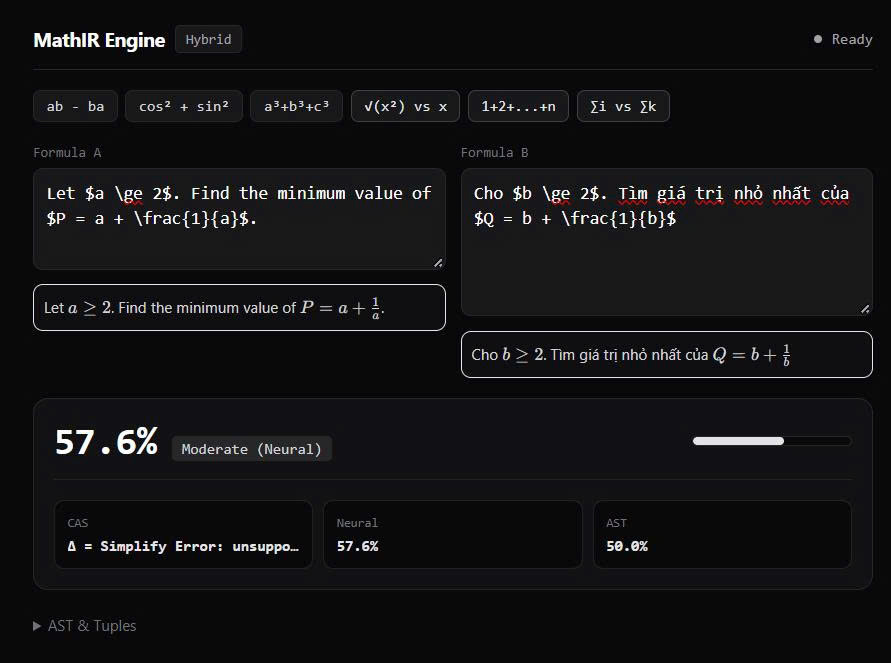
\includegraphics[width=\textwidth]{figures/fig_multilingual.jpg}
			\caption{English vs. Vietnamese query (57.6\%).}
			\label{subfig:multilingual}
		\end{subfigure}
		\hfill
		\begin{subfigure}[b]{0.485\textwidth}
			\centering
			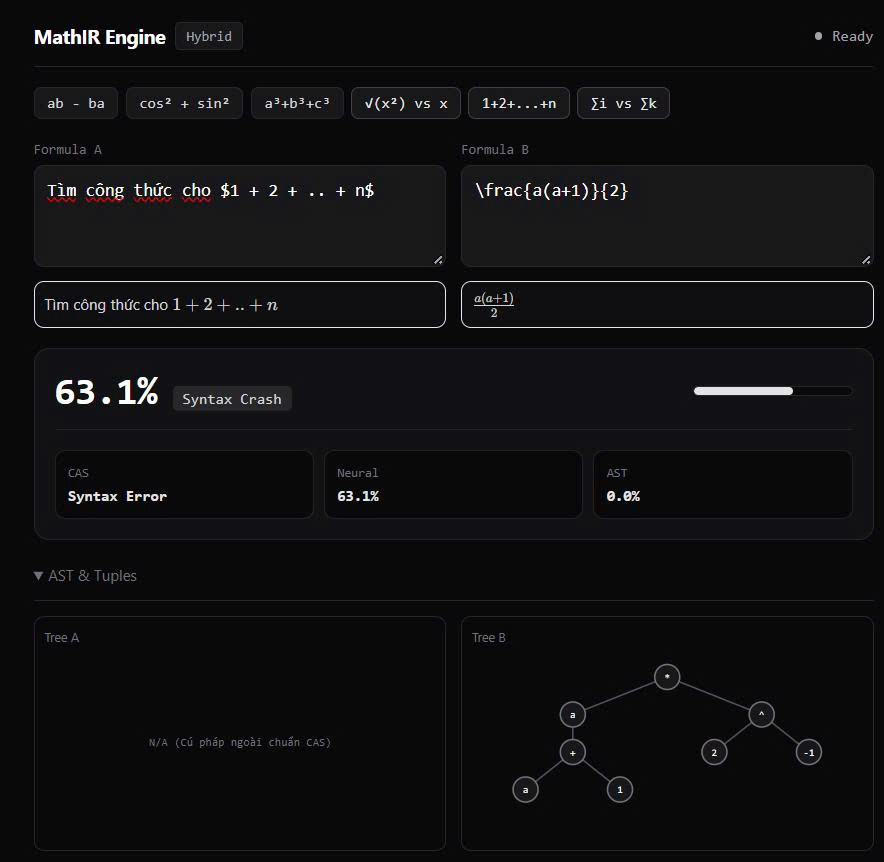
\includegraphics[width=\textwidth]{figures/fig_sequence.jpg}
			\caption{Informal sequence query ($1+2+..+n$, 63.1\%).}
			\label{subfig:sequence}
		\end{subfigure}
		\caption{Cross-lingual disparity on Vietnamese queries and failure modes on informal ellipsis syntax.}
		\label{fig:crosslingual_sequence}
	\end{figure}

	\noindent \textbf{Theoretical Cause:} Accented Vietnamese words undergo severe subword fragmentation under the English WordPiece vocabulary, scattering embedding vectors into out-of-vocabulary noise. Concurrently, CAS and AST parsers are incapable of processing non-rigorous mathematical ellipsis.

	% ==================== SECTION 3: SYMBOLIC & STRUCTURAL BASELINES ====================
	\section{Limitations of Structural and CAS Baselines}
	Detailed visual documentation is omitted for Tangent-CFT and SymPy CAS as their failure modes represent deterministic, well-documented limitations:
	
	\begin{itemize}
		\item \textbf{Tangent-CFT AST Rigidity:} The AST tuple overlap metric is hyper-sensitive to variable alpha-renaming. Substituting bound variables ($f(x) \to f(t)$) causes tuple overlap to fall to 0\%. Furthermore, evaluating algebraically equivalent structures (such as $a^2 - b^2$ vs. $(a-b)(a+b)$) yields only \textbf{25.0\%} tuple overlap due to distinct subtree depths.
		\item \textbf{SymPy CAS Syntactic Fragility:} CAS demands closed-form formal grammar. When encountering informal ellipsis sequences common in user queries ($1 + 2 + \dots + n$), the parser crashes. Similarly, CAS evaluates $\sqrt{x^2}$ vs. $x$ as distinct ($\Delta = \sqrt{x^2} - x \neq 0$) because it lacks implicit contextual domain reasoning ($x \ge 0$).
	\end{itemize}

	% ==================== SECTION 4: HYBRID ARCHITECTURE DIRECTION ====================
	\section{Proposed Research Direction: Multi-Stage Hybrid Formulation}
	The empirical evidence establishes that \textbf{no single baseline paradigm is sufficient}. We propose a \textbf{Multi-Stage Neuro-Symbolic Hybrid Architecture} that systematically combines the distinct strengths of each method (Table~\ref{tab:comparison}).

	\begin{table}[H]
		\centering
		\small
		\caption{Comparison of Baseline Strengths and Proposed Hybrid Synthesis.}
		\label{tab:comparison}
		\begin{tabularx}{\textwidth}{lXXX}
			\toprule
			\textbf{Dimension} & \textbf{MathBERT (Neural)} & \textbf{Tangent-CFT (AST)} & \textbf{Proposed Multi-Stage Hybrid} \\
			\midrule
			\textbf{Global Text Context} & High (English) / Low (Vietnamese) & None (Formula Only) & \textbf{Robust Multimodal Parsing} \\
			\textbf{Polarity Awareness} & Blind ($x>0 \approx x<0$) & Precise (AST Operators) & \textbf{Structural Penalty Gate} \\
			\textbf{Algebraic Equivalence} & Heuristic Only & Structural Only (25\%) & \textbf{CAS Deterministic Boost ($\Delta=0$)} \\
			\textbf{Retrieval Scalability} & $O(1)$ Vector Dot Product & $O(n^3)$ Tree Edit Distance & \textbf{Two-Stage Coarse-to-Fine} \\
			\bottomrule
		\end{tabularx}
	\end{table}

	\subsection{Hybrid Pipeline Design}
	\begin{enumerate}
		\item \textbf{Stage 1 (Coarse Semantic Recall):} Deploy MathBERT dense embeddings to perform high-speed vector nearest-neighbor search, filtering the top-$K$ candidate documents from the global index.
		\item \textbf{Stage 2 (Structural Penalty Verification):} Parse candidate formulas into 2D ASTs via Tangent-CFT. If opposite relational operators or inverted ratio positions are detected, a multiplicative penalty factor $\lambda \in [0.4, 0.6]$ is applied to suppress neural false positives.
		\item \textbf{Stage 3 (Deterministic Algebraic Boost):} If SymPy confirms symbolic identity ($\Delta = 0$), the document is promoted directly to Rank 1.
	\end{enumerate}

	% ==================== SECTION 5: CONCLUSION ====================
	\section{Conclusion and Next Steps}
	This benchmark report solidifies our research problem formulation for SC203. Rather than pursuing naive end-to-end model training, Group 2 focuses on an interpretable, resource-efficient Neuro-Symbolic integration. The automated benchmark test script has been open-sourced in our repository under \texttt{tests/test\_bottlenecks.py}. Our upcoming weekly milestones encompass formalizing the re-ranking penalty coefficients and evaluating retrieval efficacy on the ARQMath benchmark dataset.

\end{document}
